\documentclass[12pt, letterpaper]{../assignment}
\usepackage{graphicx}
\usepackage{courier}
\usepackage{minted}
\usepackage{amsmath}
\usepackage{polynom}
\usepackage{commath}
\usepackage{amssymb}
\usepackage{amsfonts} 
\usepackage{color}
\usepackage{cancel}
\usepackage{enumitem}
\usepackage{graphicx}
\usepackage{multirow}
\usepackage{float}
\usepackage{bm}
\usepackage{tikz}
\usetikzlibrary{shapes,arrows}
\usepackage{booktabs}
\usetikzlibrary{patterns}

% Define Theme Colors
\definecolor{light-gray}{rgb}{0.2,0.2,0.2}
\definecolor{header-blue}{rgb}{0,0,0.7}
% \definecolor{header-blue}{rgb}{0.5137,0.8353,0.9176}
\definecolor{header-blue}{rgb}{0,0.8,0.95}
\definecolor{dark-gray}{rgb}{0.1,0.1,0.1}
\pagecolor{dark-gray}
\color{white}

\usemintedstyle{monokai}
\oddsidemargin = 0pt
\exercisesheet{Module 4}{Assignment}
\student{Austin Barrilleaux}
\university{\color{header-blue}Johns Hopkins University}
\school{\color{header-blue}Whiting School of Engineering}
\courselabel{EN 535.612}
\semester{Fall 2024}
\usepackage[backend=bibtex,style=numeric,sorting=none]{biblatex}
\bibliography{reference}

\definecolor{light-gray}{rgb}{0.2,0.2,0.2}
\setminted{bgcolor=light-gray,frame=lines,rulecolor=white}
\setlength{\parindent}{0pt}

\makeatletter
\patchcmd{\minted@colorbg}{\noindent}{\medskip\noindent}{}{}
\apptocmd{\endminted@colorbg}{\par\medskip}{}{}
\makeatother

\begin{document}

\subsection*{EXERCISE 4.39}
\subsubsection*{Gear A spins relative to its shaft,
which rotates at variable rate $\bm{\Omega_1}$ about the horizontal axis.
Gear B rotates at the variable rate $\bm{\Omega_2}$.
Determine the angular velocity and angular acceleration of gear A.}

\begin{figure}[H]
    \centering
    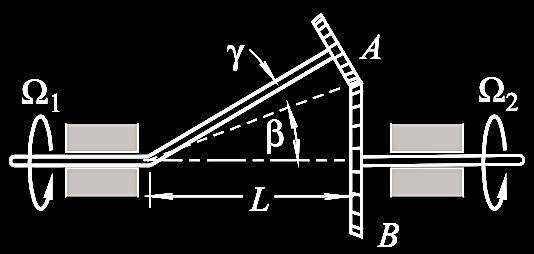
\includegraphics[frame]{images/Q4_39.png}
\end{figure}

In the following sketch, we will define two coordinate frames, $\{XYZ\}$,
$\{xyz\}$ which rotates with $\Omega_1$, and $\{x'y'z'\}$ which is rotated to align with the tilted disk from $\{xyz\}$ and rotates about the $x$-axis with $\Omega_1$:

\begin{center}
\tikzset{every picture/.style={line width=0.75pt}} %set default line width to 0.75pt        

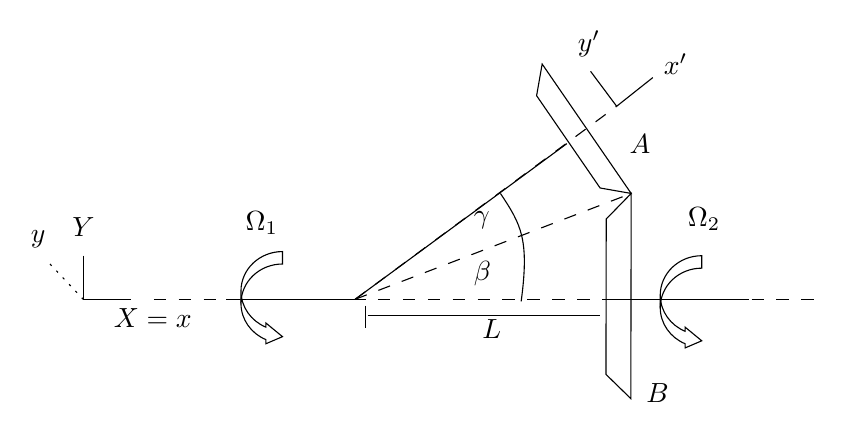
\begin{tikzpicture}[x=0.75pt,y=0.75pt,yscale=-1,xscale=1]
%uncomment if require: \path (0,300); %set diagram left start at 0, and has height of 300

%Shape: Diagonal Stripe [id:dp6584115188967272] 
\draw   (263.43,72.9) -- (266.11,57.66) -- (309,120) -- (294.03,117.37) -- cycle ;
%Shape: Diagonal Stripe [id:dp47838127500925] 
\draw   (296.98,132.31) -- (309,120) -- (308.83,218.86) -- (296.85,207.16) -- cycle ;
%Straight Lines [id:da12716113403401774] 
\draw    (114,171) -- (176,171) ;
%Straight Lines [id:da49486009433199185] 
\draw    (176,171) -- (278,96) ;
%Straight Lines [id:da8057160692207945] 
\draw  [dash pattern={on 4.5pt off 4.5pt}]  (79,171) -- (397,171) ;
%Straight Lines [id:da21369288524797425] 
\draw  [dash pattern={on 4.5pt off 4.5pt}]  (176,171) -- (302,78) ;
%Straight Lines [id:da2702667446002365] 
\draw  [dash pattern={on 4.5pt off 4.5pt}]  (176,171) -- (309,120) ;
%Curve Lines [id:da06472463066651701] 
\draw    (246,120) .. controls (256,135) and (260,142) .. (256,172) ;
%Curve Left Arrow [id:dp7426870506144505] 
\draw  [fill={rgb, 255:red, 255; green, 255; blue, 255 }  ,fill opacity=1 ] (121,167) .. controls (121,156.51) and (129.95,148) .. (141,148) -- (141,154) .. controls (129.95,154) and (121,162.51) .. (121,173) ;\draw  [fill={rgb, 255:red, 255; green, 255; blue, 255 }  ,fill opacity=1 ] (121,173) .. controls (121,180.79) and (125.94,187.49) .. (133,190.42) -- (133,192.42) -- (141,189) -- (133,182.42) -- (133,184.42) .. controls (125.94,181.49) and (121,174.79) .. (121,167)(121,173) -- (121,167) ;
%Curve Left Arrow [id:dp17263396810005305] 
\draw  [fill={rgb, 255:red, 255; green, 255; blue, 255 }  ,fill opacity=1 ] (323,169) .. controls (323,158.51) and (331.95,150) .. (343,150) -- (343,156) .. controls (331.95,156) and (323,164.51) .. (323,175) ;\draw  [fill={rgb, 255:red, 255; green, 255; blue, 255 }  ,fill opacity=1 ] (323,175) .. controls (323,182.79) and (327.94,189.49) .. (335,192.42) -- (335,194.42) -- (343,191) -- (335,184.42) -- (335,186.42) .. controls (327.94,183.49) and (323,176.79) .. (323,169)(323,175) -- (323,169) ;
%Straight Lines [id:da2528438251441085] 
\draw    (298,171) -- (366,171) ;
%Straight Lines [id:da4134757225389607] 
\draw    (182,179) -- (294,179) ;
%Straight Lines [id:da6012462634075477] 
\draw    (181,174) -- (181,185) ;
%Straight Lines [id:da5578381630289155] 
\draw  [dash pattern={on 0.84pt off 2.51pt}]  (29,154) -- (45,171) ;
%Straight Lines [id:da60365166420175] 
\draw    (302,78) -- (319.44,64.17) ;
%Straight Lines [id:da3020061529358744] 
\draw    (302,78) -- (289.44,61.17) ;
%Straight Lines [id:da5439545823041774] 
\draw    (45,171) -- (68,171) ;
%Straight Lines [id:da17805854448087177] 
\draw    (45,150) -- (45,171) ;

% Text Node
\draw (232,151.4) node [anchor=north west][inner sep=0.75pt]    {$\beta $};
% Text Node
\draw (232,127.4) node [anchor=north west][inner sep=0.75pt]    {$\gamma $};
% Text Node
\draw (307,90.4) node [anchor=north west][inner sep=0.75pt]    {$A$};
% Text Node
\draw (315,210.4) node [anchor=north west][inner sep=0.75pt]    {$B$};
% Text Node
\draw (236,179.4) node [anchor=north west][inner sep=0.75pt]    {$L$};
% Text Node
\draw (122,127.4) node [anchor=north west][inner sep=0.75pt]    {$\Omega _{1}$};
% Text Node
\draw (335,125.4) node [anchor=north west][inner sep=0.75pt]    {$\Omega _{2}$};
% Text Node
\draw (58.5,174.4) node [anchor=north west][inner sep=0.75pt]    {$X=x$};
% Text Node
\draw (38.5,130.4) node [anchor=north west][inner sep=0.75pt]    {$Y$};
% Text Node
\draw (18.5,136.4) node [anchor=north west][inner sep=0.75pt]    {$y$};
% Text Node
\draw (323.5,51.4) node [anchor=north west][inner sep=0.75pt]    {$x'$};
% Text Node
\draw (282,40.4) node [anchor=north west][inner sep=0.75pt]    {$y'$};

\end{tikzpicture}
\end{center}

We can write the angular velocity $\bar{\omega}$ as:

$$ \bar{\omega} = \Omega_1 \bar{i} + \Omega_A \bar{i}' $$

Where $\Omega_A$ is the rotation about the horizontal bar.
\\\\
We will confront this problem in the rotating $\{x'y'z\}$ frame.
The rotation from $\{xyz\}$ to $\{x'y'z'\}$ is defined by the $z$ axis rotation as:

$$ R = \left[\begin{array}{ccc}
    \cos\left(\beta +\gamma \right) & \sin\left(\beta +\gamma \right) & 0\\
   -\sin\left(\beta +\gamma \right) & \cos\left(\beta +\gamma \right) & 0\\
   0 & 0 & 1
\end{array}\right] $$

Which we can use to define:

\begin{equation*}
\begin{aligned}
    \bar{i} &= R\ \bar{i}' &= \left[\begin{array}{r} \cos\left(\beta +\gamma \right)\bar{i}'\\ -\sin\left(\beta +\gamma \right) \bar{j}' \end{array}\right] \\
    \bar{j} &= R\ \bar{j}' &= \left[\begin{array}{r} \sin\left(\beta +\gamma \right)\bar{i}'\\ \cos\left(\beta +\gamma \right) \bar{j}'\end{array}\right]
\end{aligned}
\end{equation*}

This makes:

$$ \bar{\omega} = \left[\begin{array}{r} \left\{\Omega _{A}+\cos\left(\beta +\gamma \right)\,\Omega _{1}\right\} \bar{i}'\\ \left\{-\sin\left(\beta +\gamma \right)\,\Omega _{1}\right\} \bar{j}' \end{array}\right] $$

We can solve for $\Omega_A$, by first solving for the velocity of $v_{B_{\{ijk\}}}$ relative to the rotation rate $\Omega_1$.
The rotation of $\Omega_2$ relative to $\Omega_1$ is :

$$ \Omega_{2/1} = \Omega_2 - \Omega_1 $$

Therefore:

\begin{equation*}
\begin{aligned}
v_{B_{\{ijk\}}} &= \left(\Omega_{2/1} \bar{i} \times L\tan(\beta) \bar{j}\right)\\
    &= \left\{-L\,\mathrm{tan}\left(\beta \right)\,\left(\Omega _{1}-\Omega _{2}\right)\,{\cos\left(\beta +\gamma \right)}^2-L\,\mathrm{tan}\left(\beta \right)\,\left(\Omega _{1}-\Omega _{2}\right)\,{\sin\left(\beta +\gamma \right)}^2\right\} \bar{k}' 
\end{aligned}
\end{equation*}

We can also define $v_{A_{\{ijk\}}}$ relative to the rotation rate $\Omega_1$

\begin{equation*}
\begin{aligned}
    v_{A_{\{ijk\}}} &= \Omega_A \bar{i}' \times L \frac{\sin(\gamma)}{\cos(\beta)}(-\bar{j}' )\\
        &= \left\{-\frac{L\,\Omega _{A}\,\sin\left(\gamma \right)}{\cos\left(\beta \right)} \right\} \bar{k}'
\end{aligned}
\end{equation*}

If we equate these two velocities as they are equal doe to the no slip condition, we can solve for $\Omega_A$:

$$ v_{A_{\{ijk\}}} = v_{B_{\{ijk\}}} \ \ \rightarrow  \ \
\Omega_A = \frac{\sin\left(\beta \right)}{\sin\left(\gamma \right)} \left(\Omega _{1}-\Omega _{2}\right)  $$

This makes the angular velocity $\bar{\omega}$:

\begin{answer}
$$ \bar{\omega} = \left[\begin{array}{r} \left\{ \frac{\sin\left(\beta \right)\,}{\sin\left(\gamma \right)}\left(\Omega _{1}-\Omega _{2}\right) + \cos\left(\beta +\gamma \right)\,\Omega _{1} \right\} \bar{i}'\\
    \left\{-\sin\left(\beta +\gamma \right)\,\Omega _{1} \right\} \bar{j}' \end{array}\right] $$
\end{answer}

From this, the angular acceleration $\bar{\alpha}$ is solved for as:

\begin{equation*}
    \begin{aligned}
        \bar{\alpha} &= \sum_2 \left( \dot{\omega}_n \bar{e}_n + \bar{\Omega}_n \times \omega_n \bar{e}_n \right)\\
        &= \dot{\Omega}_1 \bar{i} +
        \cancelto{0}{\Omega_1 \bar{i} \times \Omega_1 \bar{i}} +
        \dot{\Omega}_A \bar{i}' +
        \bar{\omega} \times \Omega_A \bar{j}\\
        &= \dot{\Omega}_1 \bar{i} +
        \frac{\sin\left(\beta \right)}{\sin\left(\gamma \right)} \left(\dot{\Omega}_{1}-\dot{\Omega}_{2}\right) \bar{i}' +
        \bar{\omega} \times \frac{\sin\left(\beta \right)}{\sin\left(\gamma \right)} \left(\Omega _{1}-\Omega _{2}\right) \bar{j}
    \end{aligned}
\end{equation*}

This evaluated to:
\begin{answer}
\begin{equation*}
    \begin{aligned}
        \bar{\alpha} &=
        \left[\begin{array}{r}
            \left\{\cos\left(\beta +\gamma \right)\,\dot{\Omega} _{1}+\left(\dot{\Omega}_{1}-\dot{\Omega}_{2}\right)\frac{\sin\left(\beta \right)}{\sin\left(\gamma \right)}\right\} \bar{i} \\
            \left\{-\sin\left(\beta +\gamma \right)\,\dot{\Omega} _{1}\right\} \bar{j} \\
            \left\{\sin\left(\beta +\gamma \right)\left(\Omega _{1}-\Omega _{2}\right)\,\Omega _{1}\,\frac{\sin\left(\beta \right)}{\sin\left(\gamma \right)}\right\} \bar{k} \end{array}\right]
    \end{aligned}
\end{equation*}
\end{answer}

MATLAB's symbolic toolbox was leveraged in solving this problem.
The script used to solve it is provided with the assignment submission as \texttt{Q4\_39.m}.


\subsection*{EXERCISE 4.44}
\subsubsection*{The disk rolls without slipping over the horizontal XY plane.
At the instant when $\bm{\beta = 36.87^\circ}$,
the X and Y components of the velocity of point B on the horizontal diameter of the disk are 8 m/s and -4 m/s,
respectively, and the corresponding velocity components of center A at this instant are 4 m/s and 2 m/s.
Determine the precession angle $\bm{\Psi}$ between the horizontal diameter BAC and the X axis,
and also evaluate the precession, nutation, and spin rates.}

\begin{figure}[H]
    \centering
    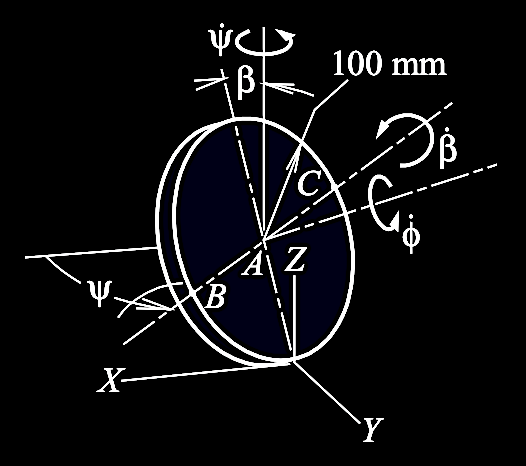
\includegraphics[scale=0.8,frame]{images/Q4_44.png}
\end{figure}

In the following sketch, we will define two coordinate frames, $\{XYZ\}$ and $\{xyz\}$:

\begin{center}

    \tikzset{every picture/.style={line width=0.75pt}} %set default line width to 0.75pt        

    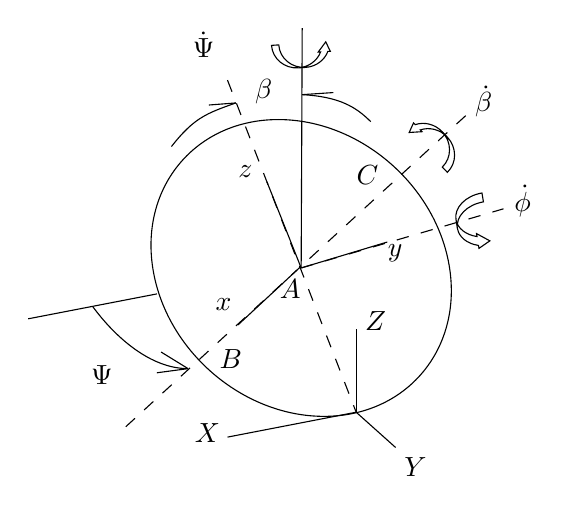
\begin{tikzpicture}[x=0.75pt,y=0.75pt,yscale=-1,xscale=1]
    %uncomment if require: \path (0,235); %set diagram left start at 0, and has height of 235
    
    %Shape: Circle [id:dp9205401865082012] 
    \draw   (163,119.5) .. controls (156.92,80.01) and (184.01,48) .. (223.5,48) .. controls (262.99,48) and (299.92,80.01) .. (306,119.5) .. controls (312.08,158.99) and (284.99,191) .. (245.5,191) .. controls (206.01,191) and (169.08,158.99) .. (163,119.5) -- cycle ;
    %Straight Lines [id:da08559310125076691] 
    \draw  [dash pattern={on 4.5pt off 4.5pt}]  (199,29) -- (261,189) ;
    %Straight Lines [id:da7745554258225504] 
    \draw    (234.5,119.5) -- (235,4) ;
    %Straight Lines [id:da5729101269761203] 
    \draw    (234.5,119.5) -- (218,78) ;
    %Straight Lines [id:da5020321684594107] 
    \draw    (199,201) -- (261,189) ;
    %Straight Lines [id:da6204394260932975] 
    \draw    (103,144) -- (165,132) ;
    %Straight Lines [id:da9164486645364178] 
    \draw  [dash pattern={on 4.5pt off 4.5pt}]  (150,196) -- (315,45) ;
    %Straight Lines [id:da7725448886535651] 
    \draw  [dash pattern={on 4.5pt off 4.5pt}]  (234.5,119.5) -- (332,91) ;
    %Curve Left Arrow [id:dp9264565990410532] 
    \draw  [fill={rgb, 255:red, 255; green, 255; blue, 255 }  ,fill opacity=1 ] (309.09,96.2) .. controls (308.14,90.42) and (313.75,84.69) .. (321.61,83.39) -- (322.32,87.67) .. controls (314.45,88.96) and (308.85,94.69) .. (309.8,100.47) ;\draw  [fill={rgb, 255:red, 255; green, 255; blue, 255 }  ,fill opacity=1 ] (309.8,100.47) .. controls (310.5,104.76) and (314.63,107.86) .. (319.92,108.64) -- (320.16,110.07) -- (325.41,106.44) -- (318.99,102.95) -- (319.22,104.37) .. controls (313.92,103.59) and (309.8,100.48) .. (309.09,96.2)(309.8,100.47) -- (309.09,96.2) ;
    %Curve Left Arrow [id:dp8307279304535069] 
    \draw  [fill={rgb, 255:red, 255; green, 255; blue, 255 }  ,fill opacity=1 ] (304.83,56.36) .. controls (309.57,61.31) and (309.62,68.95) .. (304.93,73.43) -- (302.5,70.89) .. controls (307.18,66.41) and (307.13,58.76) .. (302.39,53.81) ;\draw  [fill={rgb, 255:red, 255; green, 255; blue, 255 }  ,fill opacity=1 ] (302.39,53.81) .. controls (298.87,50.14) and (293.76,48.98) .. (289.44,50.46) -- (288.63,49.61) -- (286.55,54.23) -- (292.69,53.85) -- (291.87,53) .. controls (296.19,51.52) and (301.31,52.68) .. (304.83,56.36)(302.39,53.81) -- (304.83,56.36) ;
    %Straight Lines [id:da643022670545905] 
    \draw    (204,147) -- (232.5,120.5) ;
    %Straight Lines [id:da9284388163365738] 
    \draw    (276,107) -- (234.5,119.5) ;
    %Straight Lines [id:da801176613507065] 
    \draw    (261,189) -- (261,149) ;
    %Curve Left Arrow [id:dp5279690544622797] 
    \draw  [fill={rgb, 255:red, 255; green, 255; blue, 255 }  ,fill opacity=1 ] (233.16,23.09) .. controls (226.43,23.53) and (220.63,18.68) .. (220.22,12.26) -- (223.7,12.03) .. controls (224.12,18.46) and (229.92,23.31) .. (236.65,22.87) ;\draw  [fill={rgb, 255:red, 255; green, 255; blue, 255 }  ,fill opacity=1 ] (236.65,22.87) .. controls (241.65,22.54) and (245.76,19.39) .. (247.37,15.17) -- (248.53,15.09) -- (246.34,10.56) -- (242.72,15.47) -- (243.88,15.39) .. controls (242.27,19.62) and (238.16,22.77) .. (233.16,23.09)(236.65,22.87) -- (233.16,23.09) ;
    %Curve Lines [id:da0038494755563269756] 
    \draw    (172,61) .. controls (183,47) and (189,45) .. (203,40) ;
    %Curve Lines [id:da02069582648305146] 
    \draw    (235,36) .. controls (253,37) and (261,42) .. (268,49) ;
    %Curve Lines [id:da4975175378735417] 
    \draw    (134,138) .. controls (145,153) and (162,168) .. (180,168) ;
    %Straight Lines [id:da22471009384259655] 
    \draw    (165,170) -- (180,168) ;
    %Straight Lines [id:da9150875408939991] 
    \draw    (180,168) -- (167,160) ;
    %Straight Lines [id:da6261260756950517] 
    \draw    (190,41) -- (203,40) ;
    %Straight Lines [id:da06706977153636307] 
    \draw    (235,36) -- (250,35) ;
    %Straight Lines [id:da2976737615039562] 
    \draw    (280,206) -- (261,189) ;
    
    % Text Node
    \draw (211,27.4) node [anchor=north west][inner sep=0.75pt]    {$\beta $};
    % Text Node
    \draw (132,165.4) node [anchor=north west][inner sep=0.75pt]    {$\Psi $};
    % Text Node
    \draw (317,30.4) node [anchor=north west][inner sep=0.75pt]    {$\dot{\beta }$};
    % Text Node
    \draw (336,78.4) node [anchor=north west][inner sep=0.75pt]    {$\dot{\phi }$};
    % Text Node
    \draw (181,4.4) node [anchor=north west][inner sep=0.75pt]    {$\dot{\Psi }$};
     % Text Node
     \draw (182,193.4) node [anchor=north west][inner sep=0.75pt]    {$X$};
     % Text Node
     \draw (283,209.4) node [anchor=north west][inner sep=0.75pt]    {$Y$};
     % Text Node
     \draw (264,139.4) node [anchor=north west][inner sep=0.75pt]    {$Z$};
     % Text Node
     \draw (192,133) node [anchor=north west][inner sep=0.75pt]    {$x$};
     % Text Node
     \draw (275,107) node [anchor=north west][inner sep=0.75pt]    {$y$};
     % Text Node
     \draw (203,69) node [anchor=north west][inner sep=0.75pt]    {$z$};
     % Text Node
     \draw (260,69) node [anchor=north west][inner sep=0.75pt]    {$C$};
     % Text Node
     \draw (223,124) node [anchor=north west][inner sep=0.75pt]    {$A$};
     % Text Node
     \draw (194,157.4) node [anchor=north west][inner sep=0.75pt]    {$B$};
    
    \end{tikzpicture}
\end{center}


We can write the angular velocity $\bar{\omega}$ as:

$$ \bar{\omega} = \dot{\Psi} \bar{K} + \dot{\beta} \bar{i} + \dot{\phi} \bar{j} $$

The transformation to convert $\{XYZ\}$ to $\{xyz\}$ is:

\begin{equation*}
    \begin{aligned}
R &= \left[\begin{array}{ccc} \cos\left(\Psi \right) & -\sin\left(\Psi \right) & 0\\ \sin\left(\Psi \right) & \cos\left(\Psi \right) & 0\\ 0 & 0 & 1 \end{array}\right]
\left[\begin{array}{ccc} 1 & 0 & 0\\ 0 & \cos\left(\beta \right) & -\sin\left(\beta \right)\\ 0 & \sin\left(\beta \right) & \cos\left(\beta \right) \end{array}\right]\\
&= \left[\begin{array}{ccc} \cos\left(\Psi \right) & -\sin\left(\Psi \right)\,\cos\left(\beta \right) & \sin\left(\Psi \right)\,\sin\left(\beta \right)\\ \sin\left(\Psi \right) & \cos\left(\Psi \right)\,\cos\left(\beta \right) & -\cos\left(\Psi \right)\,\sin\left(\beta \right)\\ 0 & \sin\left(\beta \right) & \cos\left(\beta \right) \end{array}\right]
\end{aligned}
\end{equation*}

From this we see that:

\begin{equation*}
\begin{aligned}
    \bar{i} &= \left[\begin{array}{r} \cos\left(\Psi \right) \bar{I}\\ \sin\left(\Psi \right) \bar{J} \end{array}\right]\\
    \bar{j} &= \left[\begin{array}{r} -\sin\left(\Psi \right)\,\cos\left(\beta \right) \bar{I} \\ \cos\left(\Psi \right)\,\cos\left(\beta \right) \bar{J}\\ \sin\left(\beta \right) \bar{K} \end{array} \right] \\
    \bar{k} &= \left[\begin{array}{r} \sin\left(\Psi \right)\,\sin\left(\beta \right) \bar{I}\\ -\cos\left(\Psi \right)\,\sin\left(\beta \right) \bar{J}\\ \cos\left(\beta \right) \bar{K} \end{array} \right] \\
\end{aligned}
\end{equation*}

Using these, we can write the angular velocity in terms of $\{XYZ\}$:

$$ \bar{\omega} =
\left[\begin{array}{r}
    \left\{\cos\left(\Psi\right)\,\dot{\beta}-\sin\left(\Psi\right)\,\cos\left(\beta\right)\,\dot{\phi}\right\}\bar{I}\\
    \left\{\sin\left(\Psi\right)\,\dot{\beta}+\cos\left(\Psi\right)\,\cos\left(\beta\right)\,\dot{\phi}\right\}\bar{J}\\
    \left\{\sin\left(\beta\right)\,\dot{\phi}+\dot{\Psi}\right\}\bar{K}
\end{array}\right] $$

From inspection of the sketch, we can infer that:

\begin{equation*}
    \begin{aligned}
        r_{A/D} &= 0.1 \bar{k}\\
                &= \left[\begin{array}{r}
                    \left\{0.1\,\sin\left(\Psi\right)\,\sin\left(\beta\right)\right\}\bar{I}\\
                    \left\{-0.1\,\cos\left(\Psi\right)\,\sin\left(\beta\right)\right\}\bar{J}\\
                    \left\{0.1\,\cos\left(\beta\right)\right\}\bar{K}
                \end{array}\right]\\
        r_{B/D} &= 0.1 \left(\bar{k} + \bar{i}\right)\\
                &= \left[\begin{array}{r}
                    \left\{0.1\,\cos\left(\Psi\right)+0.1\,\sin\left(\Psi\right)\,\sin\left(\beta\right)\right\}\bar{I}\\
                    \left\{0.1\,\sin\left(\Psi\right)-0.1\,\cos\left(\Psi\right)\,\sin\left(\beta\right)\right\}\bar{J}\\
                    \left\{0.1\,\cos\left(\beta\right)\right\}\bar{K}
                \end{array}\right]
    \end{aligned}
\end{equation*}

Solving for the velocities at points A and B:

\begin{equation*}
    \begin{aligned}
        \bar{v}_A &= \cancelto{0}{\bar{v}_D} + \bar{\omega} \times \bar{r}_{A/D}\\
                  &= \left[\begin{array}{r}
                    \left\{0.1\,\cos\left(\beta\right)\,\left(\dot{\beta }\,\sin\left(\Psi\right)+\dot{\phi }\,\cos\left(\Psi\right)\,\cos\left(\beta\right)\right)+0.1\,\cos\left(\Psi\right)\,\sin\left(\beta\right)\,\left(\dot{\Psi }+\dot{\phi }\,\sin\left(\beta\right)\right)\right\}\bar{I}\\
                    \left\{0.1\,\sin\left(\Psi\right)\,\sin\left(\beta\right)\,\left(\dot{\Psi }+\dot{\phi }\,\sin\left(\beta\right)\right)-0.1\,\cos\left(\beta\right)\,\left(\dot{\beta }\,\cos\left(\Psi\right)-\dot{\phi }\,\sin\left(\Psi\right)\,\cos\left(\beta\right)\right)\right\}\bar{J}\\
                    \left\{-0.1\,\dot{\beta }\,\sin\left(\beta\right)\right\}\bar{K}
                \end{array}\right]\\
        \bar{v}_B &= \cancelto{0}{\bar{v}_D} + \bar{\omega} \times \bar{r}_{B/D}\\
                  &= \footnotesize \left[\begin{array}{r} 
                    \left\{0.1\,\cos\left(\beta\right)\,\left(\dot{\beta }\,\sin\left(\Psi\right)+\dot{\phi }\,\cos\left(\Psi\right)\,\cos\left(\beta\right)\right)-\left(0.1\,\sin\left(\Psi\right)-0.1\,\cos\left(\Psi\right)\,\sin\left(\beta\right)\right)\,\left(\dot{\Psi }+\dot{\phi }\,\sin\left(\beta\right)\right)\right\}\bar{I}\\
                    \left\{\left(0.1\,\cos\left(\Psi\right)+0.1\,\sin\left(\Psi\right)\,\sin\left(\beta\right)\right)\,\left(\dot{\Psi }+\dot{\phi }\,\sin\left(\beta\right)\right)-0.1\,\cos\left(\beta\right)\,\left(\dot{\beta }\,\cos\left(\Psi\right)-\dot{\phi }\,\sin\left(\Psi\right)\,\cos\left(\beta\right)\right)\right\}\bar{J}\\
                    \left\{-0.1\,\dot{\phi }\,\cos\left(\beta\right)-0.1\,\dot{\beta }\,\sin\left(\beta\right)\right\}\bar{K}
                \end{array}\right]\\       
    \end{aligned}
\end{equation*}

Given this we can set the $\bar{I}$ and $\bar{J}$ components of both velocities base on the information from the problem, as well as $\beta = 36.87^\circ$:

\begin{equation*}
    \begin{aligned}
        0.4 &= \left\{0.0640\,\dot{\phi }\,\cos\left(\Psi\right)+0.08\,\dot{\beta }\,\sin\left(\Psi\right)+0.06\,\cos\left(\Psi\right)\,\left(\dot{\Psi }+0.6\,\dot{\phi }\right)\right\}\bar{I}\\
        0.2 &= \left\{0.0640\,\dot{\phi }\,\sin\left(\Psi\right)-0.08\,\dot{\beta }\,\cos\left(\Psi\right)+0.06\,\sin\left(\Psi\right)\,\left(\dot{\Psi }+0.6\,\dot{\phi }\right)\right\}\bar{J}\\
        0.8 &= \left\{0.0640\,\dot{\phi }\,\cos\left(\Psi\right)+0.08\,\dot{\beta }\,\sin\left(\Psi\right)+\left(0.06\,\cos\left(\Psi\right)-0.1\,\sin\left(\Psi\right)\right)\,\left(\dot{\Psi }+0.6\,\dot{\phi }\right)\right\}\bar{I}\\
       -0.4 &= \left\{0.0640\,\dot{\phi }\,\sin\left(\Psi\right)-0.08\,\dot{\beta }\,\cos\left(\Psi\right)+\left(0.1\,\cos\left(\Psi\right)+0.06\,\sin\left(\Psi\right)\right)\,\left(\dot{\Psi }+0.6\,\dot{\phi }\right)\right\}\bar{J}\\
    \end{aligned}
\end{equation*}

Solving these simultaneous equations in MATLAB,
the system resolves to two different answers,
one of which matches the answer from the textbook:

\begin{answer}
\begin{equation*}
    \begin{aligned}
        \Psi &= 33.6901^\circ \\
        \dot{\Psi} &= -15.4277 \ \text{rad/s}\\
        \dot{\beta} &= 0.6934 \ \text{rad/s}\\
        \dot{\phi} &= 13.6942 \ \text{rad/s}\\
    \end{aligned}
\end{equation*}
\end{answer}

MATLAB's symbolic toolbox was leveraged heavily in solving this problem.
The script used to solve it is provided with the assignment submission as \texttt{Q4\_44.m}.

% angular acceleration α ̄

% \color{white}
% \hspace*{6em}\inputminted[frame=leftline,fontsize=\footnotesize]{matlab}
% {./matlab/B_2_18.m}
% \color{black} 

% It has the following response, which matches my analytically derived solution:

% \begin{figure}[H]
%     \centering
%     \includegraphics{matlab/B_2_18.png}
%     \caption{Response of the system}
% \end{figure}

\end{document}

